\documentclass[nometaot,lecture,amberg,autotoc,toc=twocolumn,indicatelastpageofframe,footlinebox]{OTHAWbeamer}

% Packages
\usepackage{graphicx}
\usepackage{booktabs}
\usepackage{amsmath}
\usepackage{tikz}
\usepackage{multicol}
\usepackage{array}
\usepackage{caption}
\usepackage{subcaption}

\usetikzlibrary{positioning, arrows.meta, shapes.geometric}

% Presentation Information
\title{AI CONFRENCE}
\subtitle{In-context Cascade Segmentation }

\author{Hemanthkumar}
\institution{Ostbayerische Technische Hochschule Amberg-Weiden}

\place{Amberg}
\date{\today}

\email{h.muthusamy-gunasekaran@oth-aw.de}

% Begin Document
\begin{document}

% Title Page
\maketitle

% Table of Contents
\inserttoc

% SECTION 1 — INTRODUCTION

\section{Introduction}

% Motivation
\subsection{Motivation}

\begin{frame}
    \frametitle{Why Medical Image Segmentation Matters}
    \framesubtitle{Clinical Importance}

    \begin{itemize}
        \item MRI and CT segmentation is essential for:
        \begin{itemize}
            \item Surgical planning
            \item Radiotherapy planning
            \item Disease monitoring
            \item Treatment evaluation
        \end{itemize}

        \vspace{0.5em}

        \item Manual annotation is expensive and time-consuming

        \item Sequential volumes contain many slices requiring expert labeling
    \end{itemize}

    \vspace{1em}

    % Suggested visual:
    % MRI volume or annotation workflow figure

\end{frame}

\begin{frame}
    \frametitle{Annotation Burden in Medical Imaging}
    \framesubtitle{The Core Challenge}

    \begin{block}{Problem}
        High-quality segmentation requires extensive pixel-level annotations from medical experts.
    \end{block}

    \vspace{0.8em}

    \begin{itemize}
        \item Large datasets are difficult to annotate
        \item Rare diseases have limited labeled data
        \item Annotation cost limits scalability
    \end{itemize}

    \vspace{1em}

    \centering
    \Large
    Goal: Reduce annotation requirements while maintaining segmentation quality

\end{frame}

% Problem Statement
\subsection{Problem Statement}

\begin{frame}
    \frametitle{Sequential Segmentation Problem}
    \framesubtitle{Why Slice-wise Inference Fails}

    \begin{columns}[T]

        \column{0.52\textwidth}

        \begin{itemize}
            \item Consecutive MRI/CT slices are strongly correlated

            \item Standard few-shot methods process each slice independently

            \item This leads to:
            \begin{itemize}
                \item Inconsistent boundaries
                \item Missing structures
                \item Unstable predictions
            \end{itemize}
        \end{itemize}

        \column{0.42\textwidth}

        % Suggested visual:
        % Neighboring slice inconsistency example

    \end{columns}

\end{frame}

% SECTION 2 — BACKGROUND

\section{Background}

% Medical Segmentation Evolution
\subsection{Medical Segmentation Evolution}

\begin{frame}
    \frametitle{Evolution of Medical Image Segmentation}
    \framesubtitle{From CNNs to Foundation Models}

    \begin{itemize}
        \item Traditional machine learning methods
        \item U-Net and encoder-decoder architectures
        \item Transformer-based segmentation models
        \item Foundation models for medical imaging
    \end{itemize}

    \vspace{1em}

    % Suggested visual:
    % Timeline of segmentation evolution

\end{frame}

% UniverSeg
\subsection{What is UniverSeg?}

\begin{frame}
    \frametitle{UniverSeg}
    \framesubtitle{Few-shot Medical Image Segmentation}

    \begin{itemize}
        \item Universal segmentation framework
        \item Trained on 53 medical imaging datasets
        \item Performs segmentation without additional retraining
    \end{itemize}

    \vspace{1em}

    \begin{block}{Core Idea}
        A small support set guides segmentation of unseen query images.
    \end{block}

\end{frame}

\begin{frame}
    \frametitle{UniverSeg Workflow}
    \framesubtitle{Support and Query Relationship}

    \centering

    % Insert Figure 1 here
    % \includegraphics[width=0.9\textwidth]{figures/universeg_pipeline.png}

    \vspace{1em}

    \begin{itemize}
        \item Support images contain known labels
        \item Query image is segmented using contextual guidance
        \item No fine-tuning required
    \end{itemize}

\end{frame}

% Limitations
\subsection{Limitations of Standard UniverSeg}

\begin{frame}
    \frametitle{Limitations of Slice-wise Inference}
    \framesubtitle{Missing Sequential Context}

    \begin{block}{Key Limitation}
        Standard UniverSeg does not propagate information between neighboring slices.
    \end{block}

    \vspace{1em}

    \begin{itemize}
        \item Each slice is inferred independently
        \item No memory of previous predictions
        \item Spatial continuity is not enforced
    \end{itemize}

    \vspace{1em}

    \centering
    This motivates the proposed ICS framework.

\end{frame}

% SECTION 3 — METHOD

\section{Method}

% ICS Overview
\subsection{ICS Overview}

\begin{frame}
    \frametitle{In-context Cascade Segmentation (ICS)}
    \framesubtitle{Main Idea}

    \centering

    % Insert Figure 2 here
    % \includegraphics[width=0.92\textwidth]{figures/ics_overview.png}

\end{frame}

\begin{frame}
    \frametitle{Key Concept of ICS}
    \framesubtitle{Sequential Information Propagation}

    \begin{enumerate}
        \item Start with a small labeled support set
        \item Predict neighboring slices sequentially
        \item Add predicted masks into the support set
        \item Propagate information forward and backward
    \end{enumerate}

    \vspace{1em}

    \begin{block}{Main Benefit}
        Improves inter-slice consistency without retraining.
    \end{block}

\end{frame}

% Sequential Propagation
\subsection{Sequential Propagation}

\begin{frame}
    \frametitle{Forward and Backward Inference}
    \framesubtitle{Bidirectional Segmentation}

    \begin{columns}[T]

        \column{0.48\textwidth}

        \textbf{Forward Inference}

        \begin{itemize}
            \item Predict subsequent slices
            \item Update support set continuously
        \end{itemize}

        \column{0.48\textwidth}

        \textbf{Backward Inference}

        \begin{itemize}
            \item Predict previous slices
            \item Maintain consistency in both directions
        \end{itemize}

    \end{columns}

    \vspace{1em}

    % Optional: add directional diagram

\end{frame}

% Algorithm Workflow
\subsection{Algorithm Workflow}

\begin{frame}
    \frametitle{ICS Algorithm Workflow}
    \framesubtitle{Step-by-step Procedure}

    \begin{center}
    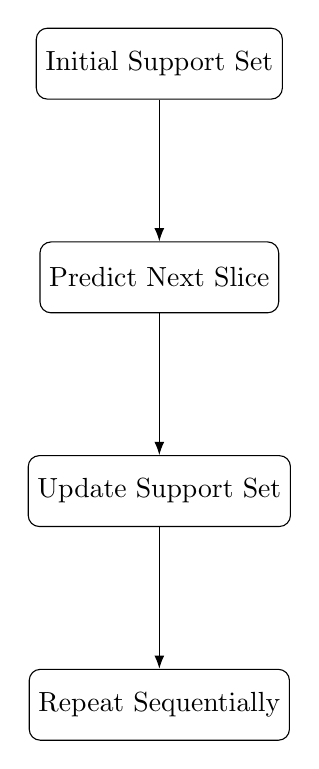
\begin{tikzpicture}[
        node distance=1.8cm,
        every node/.style={draw, rounded corners, align=center, minimum width=2.5cm, minimum height=0.9cm},
        >=Latex
    ]

    \node (start) {Initial Support Set};
    \node (predict) [below=of start] {Predict Next Slice};
    \node (update) [below=of predict] {Update Support Set};
    \node (repeat) [below=of update] {Repeat Sequentially};

    \draw[->] (start) -- (predict);
    \draw[->] (predict) -- (update);
    \draw[->] (update) -- (repeat);

    \end{tikzpicture}
    \end{center}

\end{frame}

% Why ICS Works
\subsection{Why ICS Works}

\begin{frame}
    \frametitle{Why ICS Improves Segmentation}
    \framesubtitle{Intuition Behind the Method}

    \begin{itemize}
        \item Adjacent slices contain similar anatomical structures

        \item Previously predicted masks provide contextual guidance

        \item Sequential propagation stabilizes segmentation boundaries

        \item Information continuity improves robustness
    \end{itemize}

\end{frame}

% SECTION 4 — EXPERIMENTS

\section{Experiments}

% Dataset
\subsection{Dataset}

\begin{frame}
    \frametitle{HVSMR Dataset}
    \framesubtitle{Cardiac MRI Segmentation Benchmark}

    \begin{itemize}
        \item 60 cardiovascular MRI scans
        \item 8 anatomical regions:
        \begin{itemize}
            \item LV, RV, LA, RA
            \item AO, PA, SVC, IVC
        \end{itemize}
    \end{itemize}

    \vspace{1em}

    % Suggested visual:
    % Cardiac anatomy illustration

\end{frame}

% Experimental Setup
\subsection{Experimental Setup}

\begin{frame}
    \frametitle{Experimental Setup}
    \framesubtitle{Evaluation Protocol}

    \begin{itemize}
        \item Baseline: Standard UniverSeg
        \item Metric: Dice Similarity Coefficient (DSC)
        \item Support set size varied from 1 to 5
        \item Forward and backward propagation evaluated
    \end{itemize}

\end{frame}

% SECTION 5 — RESULTS

\section{Results}

% Quantitative Results
\subsection{Quantitative Results}

\begin{frame}
    \frametitle{Quantitative Results}
    \framesubtitle{Dice Similarity Coefficient Comparison}

    \centering

    % Insert Table 1
    % Insert Figure 3

    \vspace{1em}

    \begin{block}{Observation}
        ICS significantly improves segmentation performance in several anatomical regions.
    \end{block}

\end{frame}

% Qualitative Results
\subsection{Qualitative Results}

\begin{frame}
    \frametitle{Qualitative Results: PA Region}
    \framesubtitle{Successful Sequential Consistency}

    \centering

    % Insert Figure 4

\end{frame}

\begin{frame}
    \frametitle{Qualitative Results: LV Region}
    \framesubtitle{Failure and Over-segmentation Example}

    \centering

    % Insert Figure 5

\end{frame}

% Slice Consistency
\subsection{Slice Consistency Analysis}

\begin{frame}
    \frametitle{Slice-by-Slice Consistency}
    \framesubtitle{Sequential Stability Analysis}

    \centering

    % Insert Figure 6

\end{frame}

% Ablation Studies
\subsection{Ablation Studies}

\begin{frame}
    \frametitle{Effect of Support Slice Count}
    \framesubtitle{Influence of Initial Support Size}

    \centering

    % Insert Figure 7

\end{frame}

\begin{frame}
    \frametitle{Effect of Initial Slice Position}
    \framesubtitle{Sensitivity to Initialization}

    \centering

    % Insert Figure 8

\end{frame}

% SECTION 6 — DISCUSSION

\section{Discussion}

% Strengths
\subsection{Strengths of ICS}

\begin{frame}
    \frametitle{Strengths of ICS}
    \framesubtitle{Advantages of the Proposed Method}

    \begin{itemize}
        \item Improved inter-slice consistency
        \item Reduced annotation requirements
        \item No additional retraining required
        \item Strong performance in complex anatomical structures
    \end{itemize}

\end{frame}

% Limitations
\subsection{Limitations}

\begin{frame}
    \frametitle{Limitations of ICS}
    \framesubtitle{Current Challenges}

    \begin{itemize}
        \item Error accumulation during propagation
        \item Over-segmentation in some regions
        \item Sensitivity to initial slice selection
        \item Computational cost with larger support sets
    \end{itemize}

\end{frame}

% Future Work
\subsection{Future Work}

\begin{frame}
    \frametitle{Future Directions}
    \framesubtitle{Potential Improvements}

    \begin{itemize}
        \item Confidence-aware support updates
        \item Automated support slice selection
        \item Validation on CT and ultrasound datasets
        \item Efficiency optimization and model distillation
    \end{itemize}

\end{frame}

% SECTION 7 — CONCLUSION

\section{Conclusion}

% Conclusion
\subsection{Key Takeaways}

\begin{frame}
    \frametitle{Conclusion}
    \framesubtitle{Main Takeaways}

    \begin{enumerate}
        \item ICS improves sequential medical image segmentation

        \item Propagating pseudo-support information enhances consistency

        \item The framework reduces annotation burden while maintaining strong performance
    \end{enumerate}

    \vspace{1em}

    \centering
    \Large
    ICS is a promising direction for low-annotation medical segmentation.

\end{frame}

% Thank You
\begin{thankyouframe}
\end{thankyouframe}

% BACKUP SLIDES

\appendix

\section{Backup Slides}

% Backup Slide 1
\subsection{ICS Pipeline Details}

\begin{frame}
    \frametitle{ICS Pipeline Details}
    \framesubtitle{Extended Method Overview}

    % Insert enlarged Figure 2 here

\end{frame}

% Backup Slide 2
\subsection{Dice Similarity Coefficient}

\begin{frame}
    \frametitle{Dice Similarity Coefficient (DSC)}
    \framesubtitle{Evaluation Metric}

    \[
    DSC = \frac{2|X \cap Y|}{|X| + |Y|}
    \]

    \vspace{1em}

    \begin{itemize}
        \item Measures overlap between prediction and ground truth
        \item DSC = 1 indicates perfect segmentation
        \item Higher DSC implies better performance
    \end{itemize}

\end{frame}

% Backup Slide 3
\subsection{Cardiac Anatomy}

\begin{frame}
    \frametitle{Cardiac Anatomy Labels}
    \framesubtitle{HVSMR Dataset Structures}

    \begin{itemize}
        \item LV — Left Ventricle
        \item RV — Right Ventricle
        \item LA — Left Atrium
        \item RA — Right Atrium
        \item AO — Aorta
        \item PA — Pulmonary Artery
        \item SVC — Superior Vena Cava
        \item IVC — Inferior Vena Cava
    \end{itemize}

    \vspace{1em}

    % Insert anatomy illustration here

\end{frame}

% Backup Slide 4
\subsection{Support Set Sensitivity}

\begin{frame}
    \frametitle{Support Set Sensitivity}
    \framesubtitle{Effect of Support Slice Count}

    % Insert Figure 7 here

\end{frame}

% Backup Slide 5
\subsection{Initialization Sensitivity}

\begin{frame}
    \frametitle{Initialization Sensitivity}
    \framesubtitle{Effect of Initial Slice Position}

    % Insert Figure 8 here

\end{frame}

% Backup Slide 6
\subsection{Error Propagation}

\begin{frame}
    \frametitle{Error Propagation in ICS}
    \framesubtitle{Potential Failure Mechanism}

    \begin{itemize}
        \item Incorrect pseudo-labels may propagate errors
        \item Early segmentation mistakes can accumulate
        \item Over-segmentation may affect subsequent slices
    \end{itemize}

    \vspace{1em}

    % Optional: failure visualization

\end{frame}

% Backup Slide 7
\subsection{Computational Considerations}

\begin{frame}
    \frametitle{Computational Considerations}
    \framesubtitle{Inference and Efficiency}

    \begin{itemize}
        \item ICS avoids retraining and fine-tuning
        \item Sequential inference introduces additional overhead
        \item Larger support sets increase computation
        \item Tradeoff between robustness and efficiency
    \end{itemize}

\end{frame}

% Backup Slide 8
\subsection{Method Comparison}

\begin{frame}
    \frametitle{Comparison with Alternative Approaches}
    \framesubtitle{Conceptual Comparison}

    \begin{table}
    \centering
    \begin{tabular}{lccc}
        \toprule
        Method & Sequential & Retraining & Few-shot \\
        \midrule
        U-Net & No & Yes & No \\
        UniverSeg & No & No & Yes \\
        Recurrent Models & Yes & Yes & No \\
        ICS & Yes & No & Yes \\
        \bottomrule
    \end{tabular}
    \end{table}

\end{frame}
\end{document}
